\documentclass[10pt,twocolumn,letterpaper]{article}
%% Welcome to Overleaf!
%% If this is your first time using LaTeX, it might be worth going through this brief presentation:
%% https://www.overleaf.com/latex/learn/free-online-introduction-to-latex-part-1

%% Researchers have been using LaTeX for decades to typeset their papers, producing beautiful, crisp documents in the process. By learning LaTeX, you are effectively following in their footsteps, and learning a highly valuable skill!

%% The \usepackage commands below can be thought of as analogous to importing libraries into Python, for instance. We've pre-formatted this for you, so you can skip right ahead to the title below.

%% Language and font encodings
\usepackage[english]{babel}
\usepackage[utf8x]{inputenc}
\usepackage[T1]{fontenc}
\usepackage{couriers}
\usepackage{multirow}
\usepackage{lipsum}

\usepackage{enumitem}
\newcommand{\subscript}[2]{$#1 _ #2$}

%% Sets page size and margins
\usepackage[a4paper,top=3cm,bottom=2cm,left=3cm,right=3cm,marginparwidth=1.75cm]{geometry}

%% Useful packages
\usepackage{amsmath}
\usepackage{graphicx}
\usepackage[colorinlistoftodos]{todonotes}
\usepackage[colorlinks=true, allcolors=blue]{hyperref}
\usepackage{natbib}
\bibliographystyle{unsrt}
%\bibliographystyle{plain}
%% Title
\title{
		\usefont{OT1}{bch}{b}{n}
		\normalfont \normalsize \textsc{DNDS6014 Introduction to Computational Social Science \\ Project Report Fall 2021-22} \\ [10pt]
		\huge Toxicity at Scale?\\ \Large{A Structural View of Conversation quality in political subreddits} \\
}
\selectlanguage{english}
\usepackage{authblk}
\author{Yijing Chen \\ \small{\texttt{chen\_yijing@phd.ceu.edu}}}
%\affil{\small{Central European University, Department of Network and Data Science}}

\begin{document}
\maketitle

\begin{abstract}
abstract here
\end{abstract} \\ 
\\ 
{\textbf{Keywords} \\
Social media, network analysis, political communication, friendship paradox, toxic behaviors}

\section{Introduction}

Deliberative democracy asks for efficient political communication that meaningfully engages the public in discussions of key issues. Social networking sites (SNS) provide a shared cyberspace with flexible community boundaries and topical agendas that facilitates political communication. However, virtual discussions are always as meaningfully as expected, and sometimes even become brewing sites of toxic content. 

To better understand and reflect upon the political deliberation processes that happen online, researchers need to customize analysis frameworks for different platforms with varying affordances of communication. In the field of network science, for instance, enormous amount of work have constructed who-follows-whom networks to capture the flow of information from followees to their followers \cite[e.g.,][]{conover2011political, yang2010predicting, bakshy2011everyone}. While this intuitive approach works reasonably well in characterizing users or communities on follower-following based platforms such as Twitter, it might not be the best and only option for analyzing forum-based platforms such as Reddit, where the information feed delivered to individual users are not fundamentally determined by whom they are following. 

Hence, with a focus on the toxic content in political subreddits, this project is interested in exploring creative ways to construct and interpret network models applied in the context of Reddit, and hopes to answer the overarching question: where and how toxic conversations happen online. 

More specifically, I observe toxic observations at two different levels. At the user level, I hope to answer:

\begin{enumerate}
\itemsep0em 
    \item Who talks toxically?
    \item Toxicity Paradox (TP): are my neighbors more toxic than me?
    \item Temporal Toxicity Paradox (TTP): throughout my Reddit lifespan, are my neighbors consistently more toxic than me?
\end{enumerate}

Further at the submission level, I ask the following questions:

\begin{enumerate}
\itemsep0em 
    \item How well do toxic conversations engage users?
    \item Where is the most toxic post usually located?
\end{enumerate}


%\begin{enumerate}[label=\Alph*)]% a), b), c), ...
%\item User-level
%\begin{enumerate}[label=\subscript{A}{{\arabic*}})]
%    \item Who talks toxically?
%    \item Toxicity Paradox (TP): are my neighbors more toxic than me?
%    \item Temporal Toxicity Paradox (TTP): throughout my Reddit lifespan, are my neighbors consistently more toxic than me?
%\end{enumerate}
%\item Submission-level:
%\begin{enumerate}[label=\subscript{B}{{\arabic*}})]
%    \item How well do toxic conversations engage users?
%    \item Where is the most toxic post usually located?
%\end{enumerate}
%\end{enumerate}

\section{Dataset and Preprocessing}

This project analyzes a longitudinal Reddit dataset from January 2012 to December 2015. Reddit is a hub website with many self-moderated subreddits (i.e., communities), which users can subscribe to and receive subreddit updates on their front page timelines. Within each subreddit, users can create submissions and leave comments under a submission or a comment. 

I use Pushshift API\footnote{Pushshift Reddit API documentation on GitHub: https://github.com/pushshift/api.} to collect user-generated content in 51 active political subreddits. The dataset contains over 1.4 million submissions and over 20 million comments created by more than 900 thousands unique users. Each entry is time-stamped with information about its author, textbody, net upvote score and toxicity score\footnote{Toxicity scores are assigned by Perspective API: https://www.perspectiveapi.com/.}. 

Given limited time and computational resources, I truncate the data into yearly units for analysis, and will only present the result of 2012 subset in this report, if no significant variation is noticed across years. I also filter out inactive users who have less than 100 posts (i.e., either submissions or comments) or have appeared in less than 2 unique subreddits and 10 unique submissions. For user-level analysis, I also remove submissions and comments displaying \texttt{[deleted]} in the author column or having an empty textbody, all of which are kept in submission-level analysis so that the tree graph construction can preserve the original structure of conversations as much as possible.

\begin{figure}
  \centering
  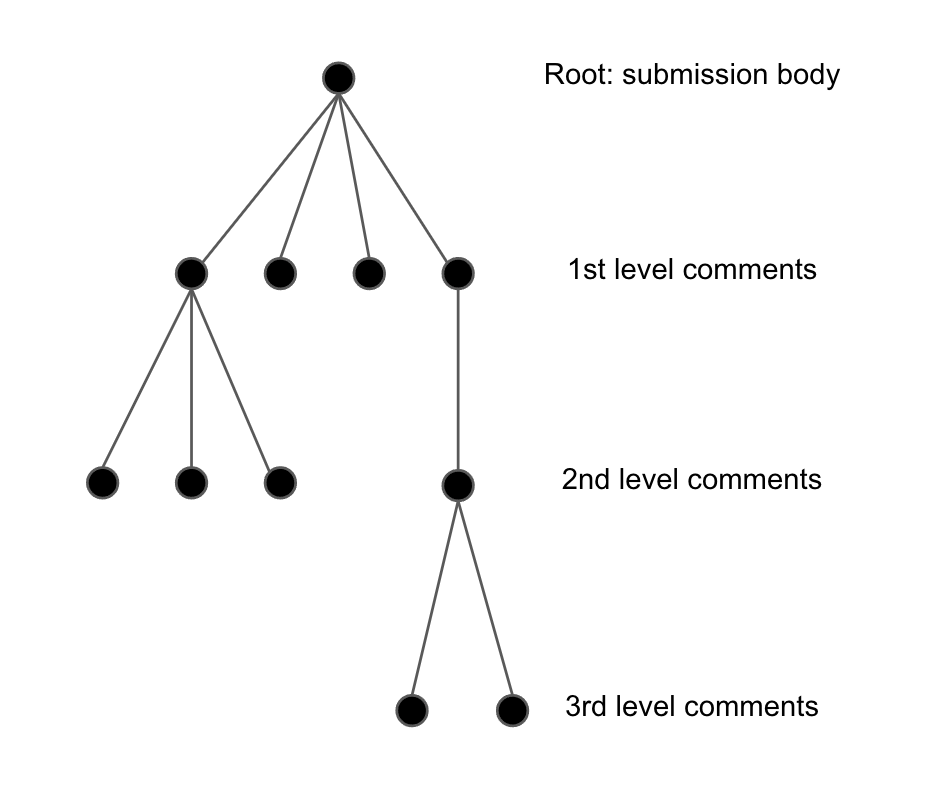
\includegraphics[width=0.4\textwidth]{figures/tree-graph.png}
  \caption{A toy example of a tree graph representation for a submission}
  \label{fig:tree-graph}
\end{figure}

\begin{figure*}[ht]
	\centering
	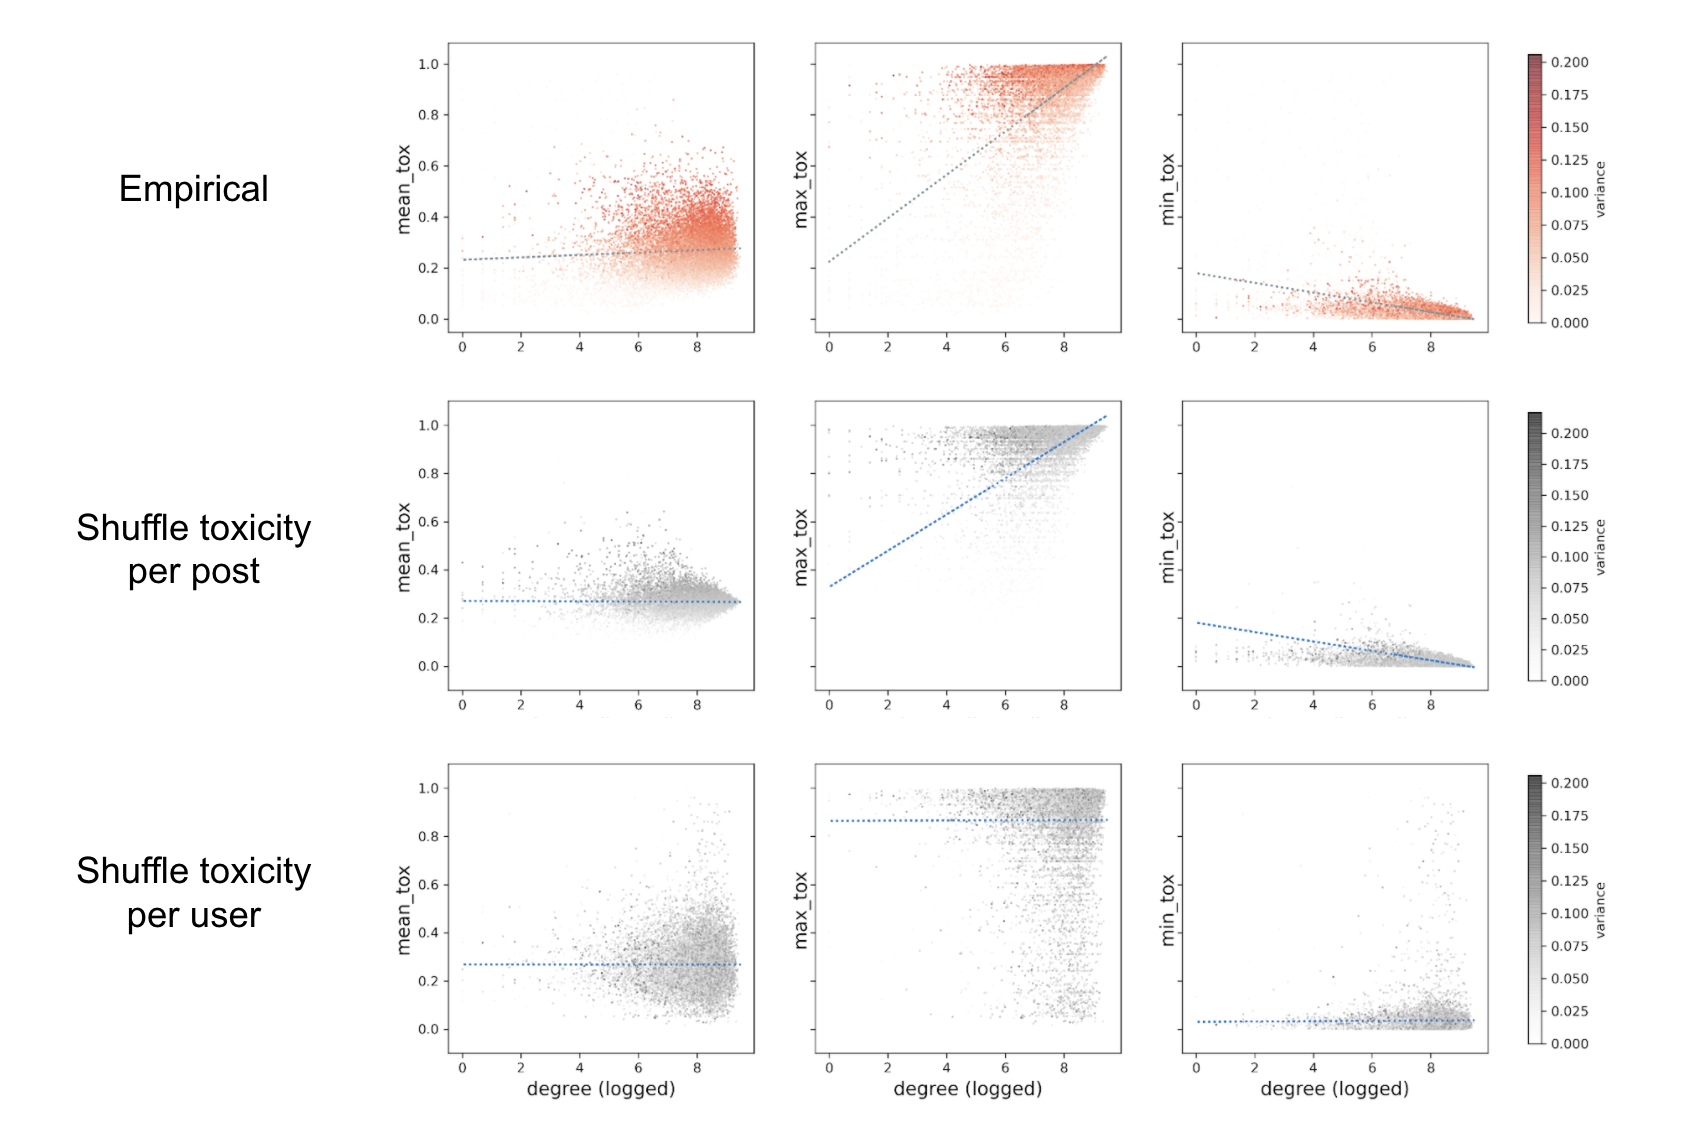
\includegraphics[width=0.9\textwidth]{figures/degree-tox.png}
	\caption{Correlation analysis of user degree and toxicity level for the empirical network and two shuffled networks. $k$ is the slope of the OLS fitting line.}
	\label{fig:degree-tox}
\end{figure*}


It is worth mentioning that, despite of the publicity of the dataset, users would not normally create the content for research purpose in particular, nor would them expect their digital traces to be made publicly identifiable. To minimize privacy risks, I only analyze and discuss the dataset in the academic setting, and make sure that personally identifiable information is either aggregated or anonymized in final results. Raw data or text content will not be released in the project repository.

\section{Methods}

\subsection{User-level analysis}

\subsubsection{User-to-user network}

I construct an undirected user-to-user graph $G_u = \{V_u, E_u\}$ where each node represents an individual user. I connect two users if they have co-appeared in the same submission at least once, assuming that they have participated in a shared conversation and have some forms of interactions, either directly through replies or indirectly through content browsing. Starting from the most basic question--who talks toxically, I use the user graph to characterize users' activity levels by node degrees, and examine the correlations between degree $d_i$ and maximum/average toxicity levels. By looking at the total number of unique neighbors a given user has shared conversations with, this measurement of activity levels positively correlates with the raw counts of submissions and comments, yet offers more nuance information about the scope of user navigation by accounting for the number of participants one have encountered along the way.

In addition to computing correlations for the empirical network, I generate two shuffled networks as null models for comparison--the first shuffling toxicity per-post and the second shuffling toxicity per-user, so that I can disentangle the effect of of varying user nature from that of pure aggregation. In other words, after empirically observing how toxicity scores distribute across user groups with varying activity levels, I wonder whether the distribution is mainly a result of the actual variation in users' toxicity levels with different navigation scopes (e.g., active users are by nature more toxic), or is simply caused by the aggregating process (i.e., active users with more posts are more likely to appear more toxic). 

\begin{figure}
  \centering
  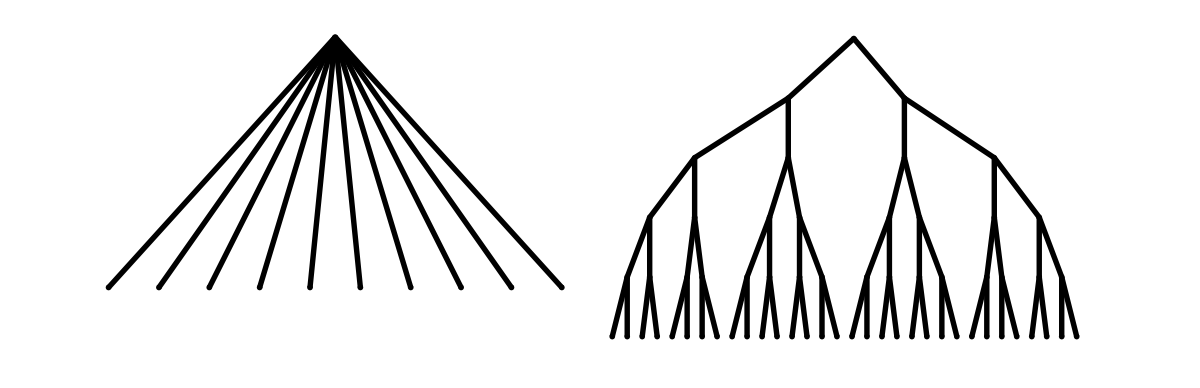
\includegraphics[width=0.4\textwidth]{figures/structural-virality.png}
  \caption{Illustrations of broadcast (left) and viral diffusion (right) \cite{goel2016structural}}
  \label{fig:structural-virality}
\end{figure}


\begin{table}[]
\centering
\begin{tabular}{l|l}
                      & Feature               \\ \hline
\multirow{2}{*}{Text} & total string length   \\
                      & average string length \\ \hline
\multirow{4}{*}{Tree} & \# of unique users    \\
                      & \# of branches        \\
                      & maximum depth         \\
                      & structural virality 
\end{tabular}
\caption{Measures of conversational engagement}
\label{tab:engagement-measure}
\end{table}


\subsubsection{Toxicity paradox: aggregated and temporal snapshots}

After individually correlating users' toxicity and activity levels, I proceed to analyze users' toxicity levels within their local neighborhood. By comparing their average toxicity scores with those of their neighbors, I investigate whether the Toxicity Paradox (TP, i.e., my neighbors are on average more toxic than me) holds true, both per node and per network. For each node, TP is true if its average toxicity $x_i$ is lower than the average toxicity of its neighbors $\mathcal{N}(i)$ \cite{eom2014generalized}, namely: 

\begin{align*}
x_i < \frac{\sum_{j \in \mathcal{N}(i)}x_j}{k_i}	
\end{align*}

For the entire network, TP is true if the expected level of toxicity across all nodes is lower than that across all neighbors \cite{eom2014generalized}, that is:

\begin{align*}
\langle x \rangle < \langle x \rangle_{nn} = \frac{\sum_{i=1}^N{k_ix_i}}{\sum_{i=1}^N{k_i}}	
\end{align*}

To stretch one step further from Eom and Jo's work on generalized friendship paradox, I examine node-level TP temporally throughout users' posting lifespan (i.e., Temporal Toxic Paradox, TTP). To operationalize, I retrieve all their posts (i.e., submissions and comments) for a given user $i$, and define the lifespan as the period of time starting from their first post and ending at their last. Then, I create a sliding window with the length of $10\%$ times their entire lifespan. Within each window, I identify all temporal neighbors $\mathcal{N}(i)^{(t)}$ of user $i$, and calculate the temporal average toxicity scores for the user and all neighbors. Similarly, for TTP to be true per node within window $t$:

\begin{align*}
x_i^{(t)} < \frac{\sum_{j \in \mathcal{N}(i)^{(t)}}x_j}{k_i^{(t)}}	
\end{align*}

\begin{table*}[ht]
\centering
\begin{tabular}{l|lll}
Network                            & Independent var. & OLS slope & Pearson's r \\ \hline
\multirow{3}{*}{empirical}         & max toxicity         & 0.0852**  & 0.4498**    \\
                                   & mean toxicity        & 0.0047**  & 0.0658**    \\
                                   & min toxicity         & -0.0191** & -0.2787**   \\
\multirow{3}{*}{shuffled per-post} & max toxicity         & 0.0785**  & 0.4168**    \\
                                   & mean toxicity        & 0.0011**  & 0.0029**    \\
                                   & min toxicity         & -0.0184** & -0.2857**  
\end{tabular}
\caption{OLS slope and Pearson's r for the empirical and per-post shuffled network (** indicates that the result is statistically significant with a p-value lower than 0.01).}
\label{tab:corr-emp-rd}
\end{table*}

\begin{table*}[ht]
\centering
\begin{tabular}{l|cccccc}
Network                   & $\rho_{kx}$ & $r_{xx}$ & $H$    & $\langle x \rangle$ &             & $\langle x \rangle_{nn}$ \\ \hline
Empirical                 & 0.0658**    & -0.0001  & 0.6170 & 0.2674              & \textless{} & 0.2724                 \\
Shuffle toxicity per post & -0.0035     & -0.0001  & 0.6170 & 0.2672              & $\approx$   & 0.2673                
\end{tabular}
\caption{Network-level toxicity paradox statistics. For both empirical and per-post shuffled network, I calculate the Pearson's r between toxicity and degree $\rho_{kx}$, the assortativity of node toxicity $r_{xx}$, the average paradox holding probability $H$, the average toxicity of nodes $\langle x \rangle$ and of neighbors $\langle x \rangle_{nn}$ (** indicates that the result is statistically significant with a p-value lower than 0.01).}
\label{tab:nw-tp}
\end{table*}

\subsection{Submission-level analysis}

\subsubsection{Submission tree graph}
For submission-level analysis, I focus on the relationship between conversational structures and toxicity levels, for which I build a tree graph to represent submission with at least one comment. As shown in Figure \ref{fig:tree-graph}, each node is a single post, and a link exists if one post is a reply to another. The depth of node indicates its nested level in a submission. 

\subsubsection{Variations of toxicity across submissions}

To measure the extent to which a submission engages a certain pool of participants, I use both textual and tree features to obtain submission-level metrics (see Table \ref{tab:engagement-measure}). For tree features in particular, apart from basic metrics such as the number of branches and maximum depth, I also consider the structural virality, a metric proposed by Goel, Anderson et al. \cite{goel2016structural} to account for both the span and the depth by calculating the average distance between all node pairs in a tree $T$, namely:

\begin{align*}
v(T) = 	\frac{1}{n(n-1)}\sum_{i=1}^n\sum_{j=1}^n d_{ij}
\end{align*}


Originally applied in analyzing diffusion trees in Twitter network, structural virality provides an interpolating measure between two extreme cases of information diffusion processes--single-generation broadcast and multi-generation spreading (see Figure \ref{fig:structural-virality}).

\begin{figure}
  \centering
  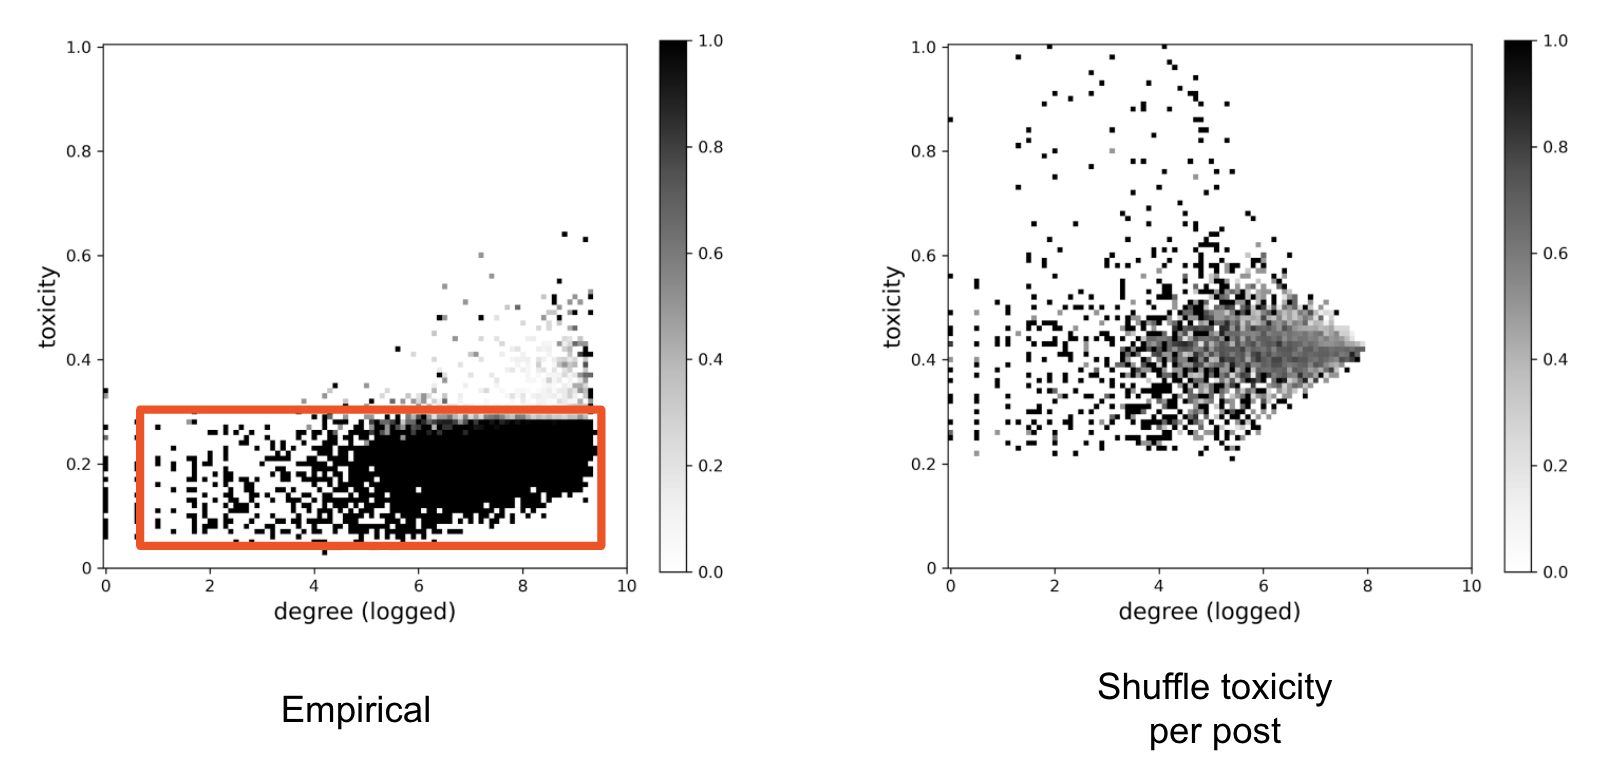
\includegraphics[width=0.49\textwidth]{figures/tp.png}
  \caption{The paradox holding probability as a function of degree and average toxicity scores.}
  \label{fig:tp-aggr}
\end{figure}


\subsubsection{Variations of toxicity within a submission}

Beyond per-tree analysis, I locate the most toxic post and see how early it occurs within a submission. Additionally, I compare the toxicity levels of parent nodes and their corresponding child nodes to examine whether there exists a generalized pattern of toxicity progression, that is, whether users tend to receive more toxic replies than their own posts.


\section{Results and Discussions}

\subsection{User-level}

\subsubsection{Who talks toxically?}

To begin with, I create Figure \ref{fig:degree-tox} to demonstrate how average, maximum, and minimum toxicity levels correlate with users' degree in both the empirical and shuffled networks. If only looking at the empirical sub-figure (top row), we may conclude that the highest toxicity levels achievable for a given user positively correlates with the number of neighbors, while average and minimum toxicity are slightly correlated but almost invariant. However, this does not necessarily imply that the more active a given user is, the more toxic the user can potentially be, and I will elaborate on breaking down the positive correlation by comparing the result against null models.

Comparing the result between the empirical the per-user shuffling network (bottom row), we can see that randomly assigning toxicity scores to individual users would flatten out all OLS fitting lines as expected, which, however, does not serve as a meaningful null model as the post-aggregation shuffling cannot inform us of possible biases that arise from the aggregation process itself. Hence, I argue that per-post shuffling that disarranges toxicity at the post level before by-user aggregation produces a better null model to compare against. Thus, I focus on comparisons between the empirical and the per-post shuffled networks and report the OLS fitting slope and Pearson's r in Table \ref{tab:corr-emp-rd}. In line with the visual impression from Figure \ref{fig:degree-tox}, two networks show fairly similar distributions of toxicity levels with respect to activity levels, with numerically close Pearson's correlation coefficients and OLS slopes. This implies that the correlation between toxicity and node degree is largely attributable to the by-user aggregation, meaning that the more posts you create, the more likely that you will have a wider range of toxicity scores with a higher ceiling and a lower floor, even when the toxicity of your posts are randomly sampled from a given pool of toxicity scores. 

\subsubsection{Toxicity paradox}

Next, I look at toxicity paradox in yearly aggregates. For node-level TP, I produce Figure \ref{fig:tp-aggr} to show the paradox holding probability $h(k,x)$ with respect to node degree $k$ and average toxicity $x$. Unlike the null result, the empirical result shows a dense TP region at the right bottom corner of the plot, implying that TP is generally true for nodes with average toxicity below 0.3 and logged degree over 4. Interestingly, we can observe a sharp horizontal division at around $x=0.3$: the paradox holding probability would drop drastically if we slide from users with toxicity levels slightly above 0.3 to those below 0.3. Such an abrupt rather than gradual decrease in $h(k,x)$ brings up an intriguing direction for future explorations. 

For network-level TP, I calculate the Pearson's r between toxicity and degree $\rho_{kx}$, the assortativity of node toxicity $r_{xx}$, the average paradox holding probability $H$, and the average toxicity of nodes $\langle x \rangle$ and of neighbors $\langle x \rangle_{nn}$. Results from the empirical and per-post shuffled networks are reported in Table \ref{tab:nw-tp}. Overall, neither of the network have an impressively high paradox holding probability, which, in accordance with Eom and Jo's finding \cite{eom2014generalized}, can be explained by the fact that the correlation between degree and average toxicity is very weak, and that the toxicity assortativity is close to zero. Comparing results from two networks, I notice that with a weaker and non-significant toxicity-degree correlation, the net difference between $\langle x \rangle$ and $\langle x \rangle_{nn}$ in null model is even smaller, which further confirms the insights from Eom and Jo's work that one origin of paradox roots in the positive correlation between degree and a given node characteristic. 

In addition to aggregated analysis, I break down TP in temporal units throughout users' lifespan and show results in Figure \ref{}


\subsection{Submission-level}

\section{Conclusions}


\section*{Acknowledgements}

The dataset was collected by the author in May 2020; the author then performed parallelized toxicity scoring jobs on University of Michigan's Great Lakes Slurm cluster, which was funded by Professor Abigail Jacobs during her work as a research assistant in summer 2020.

%{\scriptsize
%\begin{verbatim}
%\begin{figure}
%    \centering
%    \includegraphics[width=0.4\textwidth]{test.png}
%    \caption{Hello!}
%\end{figure}
%\end{verbatim}
%}

%\begin{figure}
%  \centering
%  \includegraphics[width=0.4\textwidth]{figures/test.png}
%  \caption{Notice how \LaTeX\ automatically numbers this figure.}
%\end{figure}


\bibliography{bibliography}
\end{document}
